    \documentclass[11pt]{article}
    %	options include 12pt or 11pt or 10pt
    %	classes include article, report, book, letter, thesis
    
    \title{HW4}
    \author{Shane Drafahl}
    \date{18 September ,2017}
    \usepackage{graphicx}
    \usepackage{epstopdf}
    \usepackage{graphics}

    \begin{document}
    \maketitle

    1. Let $ |x|_{a} $ be the number of occurrences of the symbol a in the string x.

    $ \newline $

    Define a context-free grammar for the language $ L = \{\ w \in \{\ 1, 0 \}\ ^{*} : |w|_{0} = |w|_{1} \}\ $

    $ \newline \newline $

    G = $ \{\ (S), (1,0), S, P  \}\ $
    $ \newline $
    $ P = \{\ $ 
    $ S \rightarrow 01 | 10 | 1S0 | 0S1 | SS | \epsilon $
    $ \}\ $

    $ \newline $

    Using a inductive proof I will give a formal proof that the grammar genderate L

    $ \newline $

    Basis: $ 01 \in \{\ 1, 0 \}\ ^{*} , 10 \in \{\ 1, 0 \}\ ^{*} $ and $ \epsilon \in \{\ 1, 0 \}\ ^{*} $
    and for all cases there are either one 1 and one 0 or zero 0 and zero 1 so they are in the language L and can be generated by G.
    $ \newline $

    IH: Suppose that A,B can be generated from G and that $ A,B \in L $

    $ \newline $

    Structural: A,B can be created from transitions from S so me must prove fro 1S0, 0S1, and SS. For SS so for
    AB or BA if we concatenated the strings A and B the 1's and 0's would still be equal because they are equal for A and B.
    For the transition 0S1 and 1S0 or 0A1 and 1A0. Its assumed by the IH that S is in L and be generated from G so A is in L and
    is generated from G. If we add a 1 and a 0 the number of 1's and 0's still equal because they do for A and adding a 1 and a 0 is still 
    equal.

    $ \newline $

    2. Define a NPDA for the language $ L = \{\ a^{n}b^{m} : m,n \in N, m \leq n \leq 2m \}\ $

    $ \newline $

    \begin{figure}[!htb]
            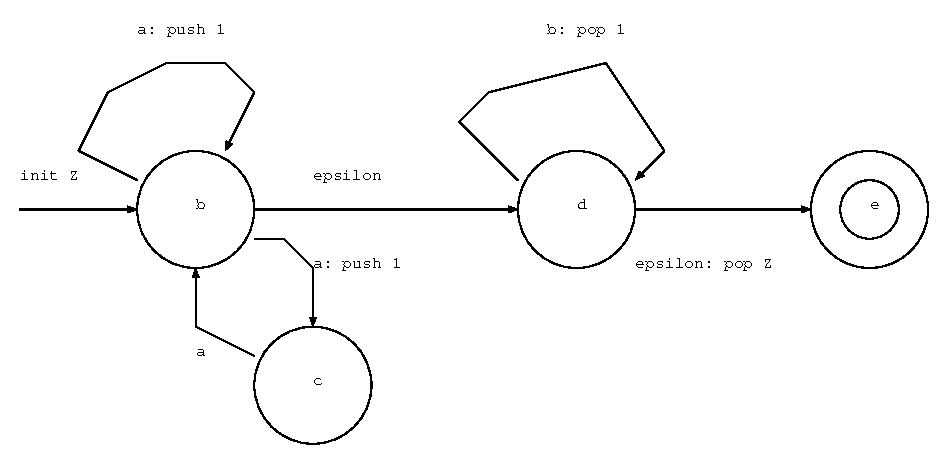
\includegraphics[scale=.7]{./hw7_pr.eps}
    \end{figure}

    $ \newline $

    3. 

    \begin{figure}[!htb]
        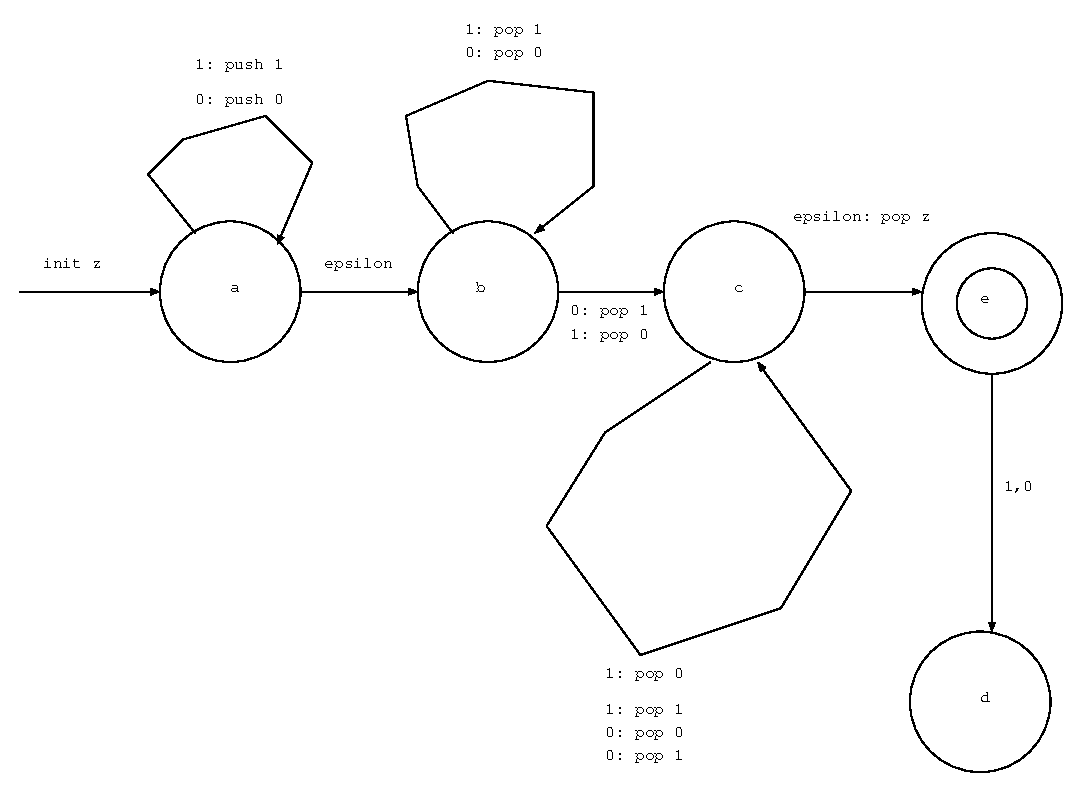
\includegraphics[scale=.7]{./hw7_2.eps}
    \end{figure}
    
    \end{document}